\documentclass[UTF8,titlepage]{article}
\usepackage{amsmath,amssymb,amsthm,amsfonts,amscd}
\usepackage{fontspec}
\usepackage{ctex}
\setmainfont{Times New Roman}
\usepackage{graphicx}
\usepackage{titlesec}
\usepackage{makecell}
\usepackage{longtable}
\usepackage{xcolor}
\usepackage{tcolorbox}
\usepackage{soul}
\usepackage{adjustbox}
\usepackage{tcolorbox}
\usepackage{enumerate}
\usepackage{pdfpages}
\usepackage{float}
\usepackage{colortbl}
\usepackage{tabularx}
\usepackage{multirow}
\usepackage{pgfplots}
\usepackage{cite}
\newcommand{\upcite}[1]{$^{\mbox{\scriptsize \cite{#1}}}$}
\numberwithin{figure}{section}
\usepackage[left=1.25in,right=1.25in,%
top=1in,bottom=1in]{geometry}
\usepackage{color}
\titleformat{\section}
  {\raggedright\LARGE\bfseries}{\thesection}{1em}{}
\begin{document}
\title{人工智能专业导论报告\\{\Large NeRF技术综述}}
\author{赵伯远 211440128}
\date{\today}
\maketitle
\tableofcontents
\clearpage
\section{神经辐射场(Neural Radiance Fields) }
\subsection{概论}

计算机视觉研究中探索的主要问题之一是视图合成,它在计算机图形和三维渲染领域有许多影响和共享方法。这个问题的解决方案旨在开发一种方法,能够在给定来自稀疏视点集的二维RGB图像输入的情况下生成特定场景的新视图。这样一个模型的输出应该在一个连续的视点集上进行采样,从而产生同一场景的真实的新视图。一些流行的方法包括光场插值,通过基于网格的近似进行表面估计,以及最近的神经体积渲染(基于神经网络的方法)。神经辐射场(NeRF)是由Mildenhall等人提出的,属于后一类方法,使用神经网络架构来表示场景,并使用神经体积渲染来合成新的视图,以达到最优效果。原始论文\upcite{mildenhall2020nerf}普及了NeRF作为视图合成的突出方法,并做出了3个总体贡献,使该框架能够产生逼真的输出,能够对场景的复杂形状和表示进行建模。(1)第一个贡献是通过一个简单的全连接神经网络来表示一个连续的场景,该网络将5D输入(3个欧氏坐标维度和2个观察方向维度)映射到4D输出(RGB颜色通道和体积密度)。(2) 第二个贡献是使用神经体积渲染技术,利用可微分的相机射线,使优化RGB表示成为可能。(3)最后,利用位置编码技术将输入域转化为更高维的空间,这使得神经网络在训练过程中能够捕捉到场景表示中更高频率的细节。此后,NeRF模型得到了改进和扩展,以捕捉各种模式的表征。

\subsection{神经立体渲染(Neural Volume Rendering)}

NeRF表示法是基于神经体积构建的,这是一种隐式的3D场景表示,通过深度神经网络的权重进行学习和存储。在Lombardi等人的研究中\upcite{Lombardi:2019},2D图像被输入到变分自编码器(VAE)中,并被编码为潜在代码。解码器的输出将潜在代码重构为体积体素表示,每个空间点都有一个RGB和alpha通道的复合表示。虽然他们的研究目标是从2D图像构建3D表示,但VAE是通过使用射线行进技术对体素表示进行2D图像重构来训练的。射线行进是一个可微过程,使得使用梯度下降方法进行优化成为可能。可以通过估计从给定视角的3D场景投影到图像平面的每个像素的辐射值来执行场景的2D重构。

每个像素位置的射线在与图像/相机平面垂直的给定视角下投影到3D空间,并用于表示沿射线的空间的体积或占用情况。像素的体积密度是通过沿射线取体积的积分来确定的;这个过程被称为体积渲染。由于在计算上无法确定沿连续射线的体积,因此沿射线的离散点的体积被采样以估计积分;这种用于体积渲染的技术被称为射线行进。像素的辐射和体积通常在重构的2D图像中表示为颜色(r,g,b)和不透明度。这个过程可以通过神经网络进行映射,这种表示方法的全部被称为神经体积渲染。

在Lombardi等人的案例中,神经体积渲染被用来从VAE的输出中重构从3D体素输出获得的图像。然而,由于VAE的性质,当从低维空间的潜在代码被上采样到高维的3D体素空间时,会出现伪影和重构扭曲。需要应用各种额外的技术来减轻这些影响。因此,最终的3D形状几何形状通常不够完美。相比之下,视图合成的目标是从新的视点生成逼真的图像。使用VAE来重构3D体素解释是不必要的,因为它会导致在\cite{Lombardi:2019}中描述的有缺陷的表示。

\begin{figure*}[t]
  % ensure that we have normalsize text
  \normalsize
  
  \centerline{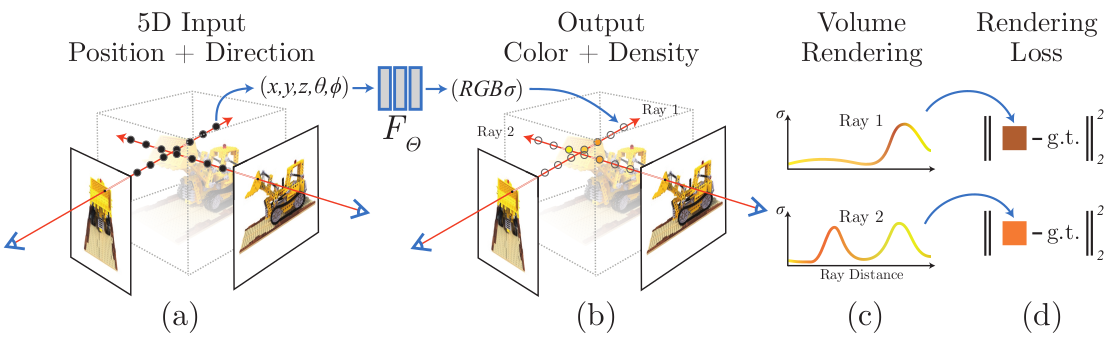
\includegraphics[scale=0.35]{fig.png}}
  \caption{NeRF场景表示流程概述。 (a) 5D输入的前馈传递。 (b) 4D输出在2D空间的映射。 (c) 射线行进进行体积渲染。 (d) 优化重构损失。 \upcite{mildenhall2020nerf}}
  \label{nerf}
  % The spacer can be tweaked to stop underfull vboxes.
\end{figure*}

\subsection{3D场景表示}

原始的NeRF论文提出,场景的表示应该是一个神经体积,由一个简单的全连接神经网络架构的权重描述,这种架构被称为多层感知器(MLP),其5D输入 $(x,y,z,\theta, \Phi)$ 对应于3D空间中的一个位置,$x=(x,y,z)$ 和2D视角,$d=(\theta, \Phi)$,这对应于相机射线上的一个点。MLP的输出对应于在该视点的2D图像平面上的像素的颜色通道,$c=(r,g,b)$ 和体积密度,$\sigma$ 的映射。

与前一项研究不同,场景的3D表示完全通过简单的前馈MLP的权重隐式表示,而不是通过体素表示。MLP前馈网络可以表示为 $F_{\Theta}:(x,d) \rightarrow (c,\sigma)$。MLP的参数$\Theta$通过一个可微的体积渲染函数进行优化,并在一组已知视角的真实图像上进行训练。损失函数可以通过评估真实像素颜色和体积渲染过程中预期像素颜色之间的差异来选择。在论文中,作者使用了一个简单的均方误差。关于原始论文中NeRF场景表示的视觉概述,请参见图\ref{nerf}\upcite{mildenhall2020nerf}。

\subsection{位置编码(Positional Encoding)}

当按照上一节所述直接训练MLP,$F_{\Theta}:(x,d) \rightarrow (c,\sigma)$,模型往往难以输出精细的结果。这是许多编码任务中的一个常见问题,其中一个希望通过全连接神经网络的权重来编码一个表示方法(如图像)。这个任务很困难,因为MLP倾向于更快地学习低频信号。然而,由于神经体积渲染的目标是将一个精确的几何形状拟合到一个3D场景,所以最好让网络过拟合数据。 Tancik等人\upcite{tancik2020fourfeat}引入了一种在变换器中常用的方法,称为位置编码,将低频输入映射到高频域。将输入映射到高频域使MLP能够捕捉到场景中的高频和高分辨率细节。当应用到MLP时,NeRF模型变为$F_{\Phi}:(\gamma(x),\gamma(d)) \rightarrow (c,\sigma)$。其中$\gamma(.)$是将我们的输入映射到高频域的函数。在NeRF的情况下,使用傅里叶特征映射作为高频特征映射函数。

\subsection{NeRF的内在属性}

NeRF模型及其视图合成的优化方法已被描述为一种可以捕获3D场景的高频几何细节的神经体积表示。这给NeRF一些有趣的内在属性,超越了视图合成的任务。首先要注意的是,由于3D几何表示被存储为全连接神经网络内的权重,NeRF可以被视为3D模型的压缩格式。3D模型可以通过查询预训练的NeRF在预定义的视点上,然后应用3D几何构造方法如行进立方体来重构。这很重要,因为NeRF文件的大小会小于模型训练的单个图像。第二个属性是NeRF捕获了关于场景的关系几何信息。这使我们能够使用详细的几何信息进行如生成深度图和形状可视化等任务。这也可以用来捕获混合现实场景的遮挡效果。第三个属性是在不同视角下可视化颜色感知效果的能力。这个属性允许在固定位置下以逼真的方式捕捉各种照明条件下的场景。

\subsection{意义与挑战}

从NeRF方法中得到的视点结果非常详细,并在合成模型的场景和真实场景中都超过了先前的最优方法。然而,到目前为止描述的原始NeRF模型在现实世界的实现中有几个限制。我们将首先关注的是训练和优化过程。实现NeRF模型的挑战在于,每个场景都需要在已知视点方向的图像上进行训练。虽然这个问题对于即时应用似乎相当限制,但存在一些方法可以估计这些参数,包括COLMAP结构从运动包\upcite{schoenberger2016sfm}。这可能在生成新场景时引入一些变化,尽管如此,得到的结果仍然相当令人印象深刻。训练和渲染过程比其他方法慢得多,需要从独特视点的多样化图像集来捕捉无缝连续的视图合成。大多数实现至少需要80张图像进行训练。用非常稀疏的图像训练的模型将生成无法解释的场景,并且无法推广。其他挑战包括被捕捉的场景的限制。NeRFs被限制在静态场景,因为动态因素的影响可能对视图合成产生剧烈的影响。这包括反射、移动的物体和背景。原始模型观察到的这些挑战已经创造了一个新的研究领域,专门针对优化和扩展基础NeRF概念。

\section{心得体会}

我最初接触人工智能的相关算法是在初中的时候,当时为了解决最短路问题,在普遍使用Dijkstra算法的同时,我尝试了一下A*算法,虽然在当时的样例数据下并无明显优势,但是我对于A*这种启发式算法的思想产生了兴趣,并在之后自行学习了一系列基本的机器学习算法。

到了大学我开始接触深度学习领域(主要是因为上大学之后手里有钱租服务器了……),上手的第一个项目是YOLOv5\upcite{couturier2021deep},当时我对于深度学习的理解还停留在“神经网络就是一个黑盒子,输入数据,输出结果”的阶段,对于YOLOv5的代码我只是简单地修改了一下数据集,然后就开始训练了,结果是,我在服务器上训练了一个星期,最后的结果还不如YOLOv5的预训练模型。于是我和我的队友回去重新阅读了原始论文\cite{couturier2021deep}, 开始理解一些概念,比如说数据增强、损失函数、激活函数等等,也开始尝试修改网络结构,使得模型可以部署在gpu较弱的NUC上。在这个过程中非常感谢隗兵老师和唐雪嵩老师给我提供的建议和帮助,帮我们解决了不少问题。最终我们的修改的YOLOX\upcite{ge2021yolox}模型在NUC上的推理速度达到了35fps(CPU)和100fps(核显)。

对NeRF技术的研究始于本学期初接触了3D重建的相关领域,但是由于时间原因研究还不是非常深入,正好借此机会做一些简单的技术总结。在此过程中非常感谢李大威老师的帮助与指导。我相信未来NeRF技术会在更多的领域发挥作用。

\section{未来规划}
\subsection{对于NeRF技术}

NeRF研究的最新发展解决的一个挑战领域是场景的校准过程。由于训练和渲染新场景的时间和计算密集过程,NeRF的实现往往受到限制。目前相关的研究有RegNeRF\upcite{Niemeyer2021Regnerf}、FreeNeRF\upcite{yang2023freenerf}等,我目前正在基于FreeNeRF的代码进行研究,希望能够在未来的研究中对NeRF技术有更深入的理解,将其应用在更多领域中。

\subsection{对于个人}

未来考虑在学习专业知识的基础上,学习神经科学和认知科学,让神经网络可解释化,

专业方向上目前仍考虑以CV和DL为主,希望未来能做出足够有趣的作品。

反正不打算改行。
\clearpage
\bibliographystyle{ieeetr}
\bibliography{references}
\vspace{12pt}

\end{document}